\subsubsection{Flöde vid termisk jämvikt}



%To regerenate the figures use /code/pdesolver/generateWallFigApril.m
%with the argument /code/pdesolver/walldata.mat
\begin{figure}
\centering

\subfloat[Energiflöde ut från insidan av en vägg med $0,5\mbox{m}$ tegel.]{
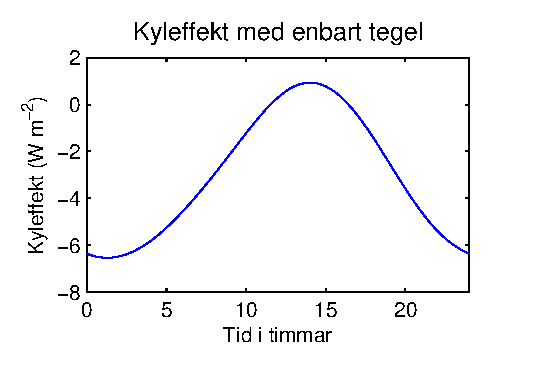
\includegraphics[width=6cm]{images/noinsulationapril.eps}
}\vspace{5mm}
\subfloat[Energiflöde ut från insidan av en vägg med $0,5\mbox{m}$ tegel och
$1\mbox{dm}$ tilläggsisolering bestående av mineralull.]{
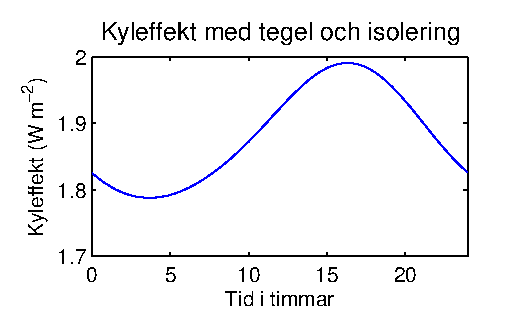
\includegraphics[width=6cm]{images/insulationapril.eps}
}
\caption{Energiflödena är tagna från en fiktiv dag som skulle motsvara en molnfri
15 april 2011. Här har temperaturen varierat mellan 6 grader Celsius på natten och
9 grader Celsius på natten. Beräkningen är genomförd med finita elementmetoden där
temperaturen på insidan av väggen satts till konstanta 20 grader Celsius.}
\end{figure}
